\documentclass[conference]{IEEEtran}
\usepackage{times}

% numbers option provides compact numerical references in the text. 
\usepackage[numbers]{natbib}
\usepackage{multicol}
\usepackage[bookmarks=true]{hyperref}

\usepackage[pdftex]{graphicx}
\usepackage{comment}

\usepackage{algorithm}
\usepackage[noend]{algpseudocode}

\usepackage{amsthm}
\newtheorem{thm}{Theorem}
\newtheorem{lem}{Lemma}

\pdfinfo{
   /Author (Homer Simpson)
   /Title  (Robots: Our new overlords)
   /CreationDate (D:20101201120000)
   /Subject (Robots)
   /Keywords (Robots;Overlords)
}

\begin{document}

% paper title
\title{ MORRF$^{*}$ : Sampling-Based Multi-Objective Motion Planning }

% You will get a Paper-ID when submitting a pdf file to the conference system
\author{Author Names Omitted for Anonymous Review. Paper-ID [add your ID here]}

\maketitle

\begin{abstract}
The abstract goes here.
\end{abstract}

\IEEEpeerreviewmaketitle

\begin{comment}
Final Paper Submission Deadline: January 22, 2015, 23:59 PST

Papers can be up to 8 pages + references. 
This means that if more than 8 pages are used, the 9th and subsequent pages should contain ONLY references. 
The length requirement will be strictly enforced.
\end{comment}

\begin{comment}


\end{comment}

\section{Introduction}
\label{sec:intro}

\begin{comment}
(1) Why the multi-objective path planning is needed 
(2) Why the multi-objective path planning is hard (compare with a common multi-objective optimization problem)
\end{comment}

\section{Related works}
\label{sec:related_works}

\begin{comment}
(1) multi-objective  
(2)
\end{comment}

\section{Multi-Objective Rapidly exploring Random Forest$^{*}$}
\label{sec:morrt}

\subsection{Decomposition based multi-objective optimization}


\begin{thm}
\label{thm:moo-d:rrt}
The decomposition method is applicable to a RRT structure.
\begin{proof}
Let the path from start to goal with the most vertices be $ N $ segments.
Any other paths can be represented into $ N $ segments (because they have less than $ N $ segment).
By this way, all the paths could be mapped into a $ N $ dimensional space.
\end{proof}
\end{thm}

Given a multi-objective optimization problem with $ K $ objectives,
there are $ K $ objectives to be minimized. 
By Theorem \ref{thm:moo-d:rrt}, it can be decomposed into $ N $ subproblems.

Two types of tree structure are used for the optimization process.
\begin{itemize}
\item Each \emph{reference tree} explores for a single objective $ f_{k} (x), k \in K $. 
\item Each \emph{subproblem tree} explores for a subproblem $ g_{n} ( x \mid \lambda_{n} , z^{*} ) , n \in N $.
\end{itemize}

Like all the sampling-based optimization, the random positions are uniformly sampled from the workspace.
It means that all the tree have equivalent vertices constructed from same positions set sequentially.
But they are connected by different measurements of the costs, either a single objective or a cost from subproblem definition.
The edges of the trees can be different.

\begin{figure}[H]
\centering
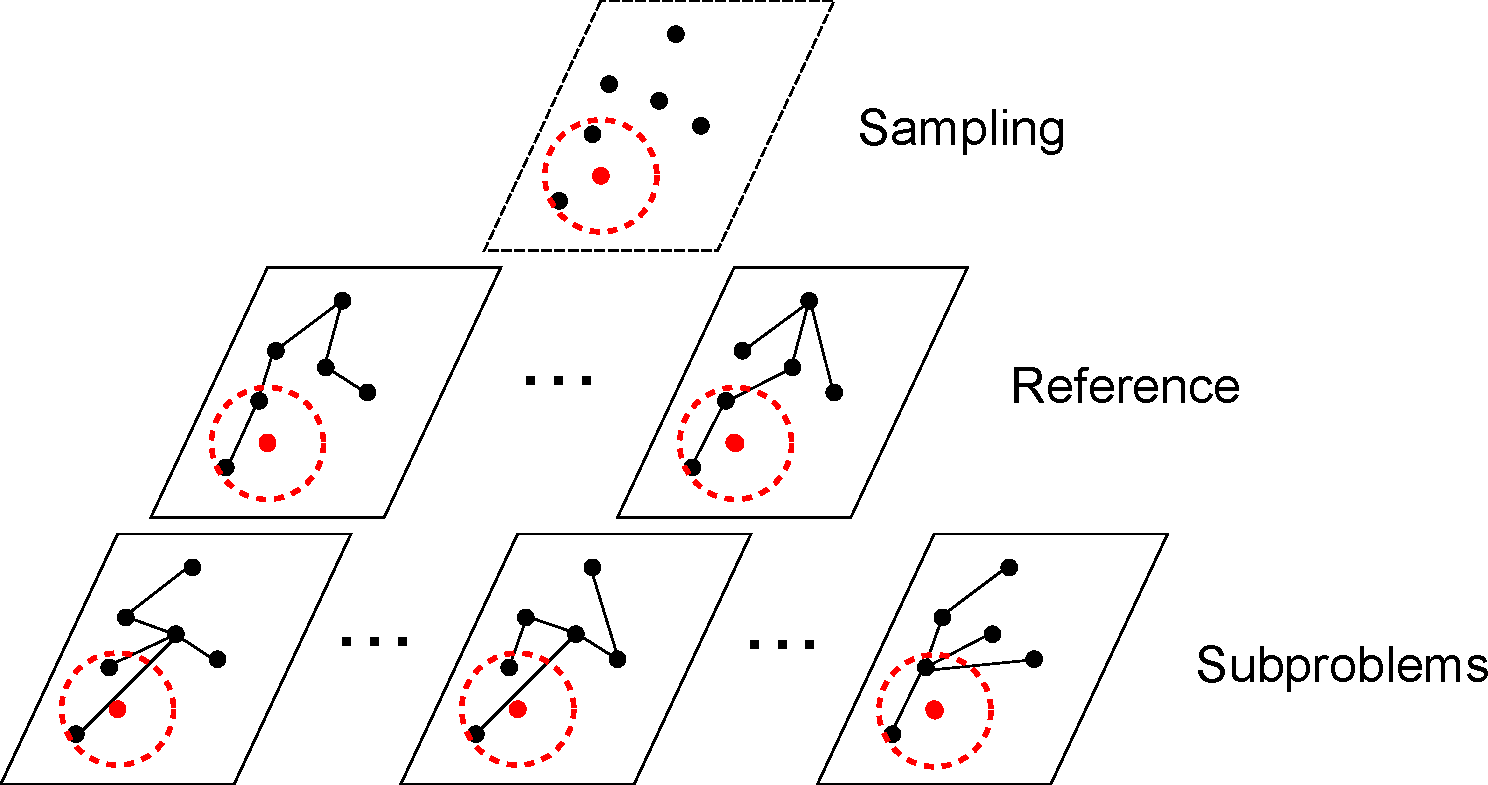
\includegraphics[width=0.9\linewidth]{./fig/MORRTstar}
\caption{Rapidly Exploring Process}
\label{fig:MORRTstar}
\end{figure}


\begin{algorithm}
\begin{algorithmic}[1]
\For{ \textbf{each} $ V_{r} \in \mathbf{V}_{r} $ } 
	\State $ V_{r} \leftarrow \{ x_{init} \} $; $ E_{r} \leftarrow \emptyset $; $ i \leftarrow 0 $
\EndFor
\For{ \textbf{each} $ V_{s} \in \mathbf{V}_{s} $ } 
	\State $ V_{s} \leftarrow \{ x_{init} \} $; $ E_{s} \leftarrow \emptyset $; $ i \leftarrow 0 $
\EndFor
\While{ $ i < N $ }
	\For{ \textbf{each} $ G_{r} \in \mathbf{G}_{r} $ } 
		\State $ G_{r} \leftarrow (V_{r}, E_{r}) $
	\EndFor
	\For{ \textbf{each} $ G_{s} \in \mathbf{G}_{s} $ } 
		\State $ G_{s} \leftarrow (V_{s}, E_{s}) $
	\EndFor
	\State $ x_{rand} \leftarrow $ \Call{ Sample }{$ i $} ; $ i \leftarrow i + 1 $
	\State $ V' \leftarrow V $; $ E' \leftarrow E $
	\State $ x_{nearest} \leftarrow $ \Call{Nearest}{$ G, x $}
	\State $ x_{new} \leftarrow $ \Call{Steer}{$ x_{nearest}, x $}
	\If{ \Call{ObstacleFree}{$ x_{nearest}, x_{new} $} }
		\For{ \textbf{each} $ G_{r} \in \mathbf{G}_{r} $ } 
		\State $ (V_{r}, E_{r}) \leftarrow $ \Call{ Extend$_{Ref}$ }{$ G_{r}, x_{new} $}
		\EndFor
		\For{ \textbf{each} $ G_{s} \in \mathbf{G}_{s} $ } 
		\State $ (V_{s}, E_{s}) \leftarrow $ \Call{ Extend$_{Sub}$ }{$ G_{s}, x_{new} $}
		\EndFor
	\EndIf
\EndWhile
\end{algorithmic}
\label{alg:rapidly_exploring_process}
\caption{Multi-objective Rapidly Random exploring }
\end{algorithm}

\begin{algorithm}
\begin{algorithmic}[1]
\State $ V' \leftarrow V' \cup \{ x_{new} \} $
\State $ x_{min} \leftarrow x_{nearest} $
\State $ X_{near} \leftarrow $ \Call{Near}{$ G, x_{new}, | V | $}
\For{\textbf{each} $ x_{near} \in X_{near} $ }
	\If{ \Call{ObstacleFree}{$ x_{new} , x_{near} $} }
		\State $ c_{k}' \leftarrow $ \Call{Cost$_{k}$}{$ x_{near} $} $ + c_{k}( $ \Call{Line}{$ x_{near}, x_{new} $} $ ) $ 
		\If{ $ c_{k}' < $ \Call{Cost$_{k}$}{$ x_{new} $} }
		\State $ x_{min} \leftarrow x_{near} $
		\EndIf
	\EndIf
\EndFor
\State $ E' \leftarrow E' \cup \{ ( x_{min}, x_{new} ) \} $
\For{\textbf{each} $ x_{near} \in X_{near} \setminus \{ x_{min} \} $ }
	\If{\Call{ObstacleFree}{$ x_{new} , x_{near} $}}
	    \State $ c_{k}' \leftarrow $ \Call{Cost$_{k}$}{$ x_{new} $} $ + c_{k}( $ \Call{Line}{$ x_{new}, x_{near} $} $ ) $ 
	    \If{ $ c_{k}' < $ \Call{Cost$_{k}$}{$ x_{near} $} }
			\State $ x_{parent} \leftarrow $ \Call{Parent}{$ x_{near} $}
			\State $ E' \leftarrow E' \setminus \{ ( x_{parent}, x_{near} ) \} $
			\State $ E' \leftarrow E' \cup \{ ( x_{new}, x_{near} ) \} $
		\EndIf
	\EndIf
\EndFor
\Return $ G' = (V', E') $ 
\end{algorithmic}
\label{alg:morrtstar:extend:ref}
\caption{ $ \mbox{Extend}_{Ref} (G, x) $}
\end{algorithm} 

\begin{algorithm}
\begin{algorithmic}[1]
\State $ V' \leftarrow V' \cup \{ x_{new} \} $
\State $ x_{min} \leftarrow x_{nearest} $
\State $ X_{near} \leftarrow $ \Call{Near}{$ G, x_{new}, | V | $}
\For{\textbf{each} $ x_{near} \in X_{near} $ }
	\If{ \Call{ObstacleFree}{$ x_{new} , x_{near} $} }
		\State $ \vec{c}' \leftarrow $ \Call{Cost}{$ x_{near} $} $ + \vec{c}( $ \Call{Line}{$ x_{near}, x_{new} $} $ ) $ 
		\State $ \eta' =  $ \Call{Fitness}{ $ \vec{c}' , \vec{c}^{*} \mid \lambda_{G} $ }
		\State $ \vec{c}_{new} = $ \Call{Cost}{$ x_{new} $} 
		\State $ \eta_{new} = $ \Call{Fitness}{ $ \vec{c}_{new} , \vec{c}^{*} \mid \lambda_{G} $ }
		\If{ $ \eta' < \eta_{new} $ }
			\State $ x_{min} \leftarrow x_{near} $
		\EndIf
	\EndIf
\EndFor
\State $ E' \leftarrow E' \cup \{ ( x_{min}, x_{new} ) \} $
\For{\textbf{each} $ x_{near} \in X_{near} \setminus \{ x_{min} \} $ }
	\If{\Call{ObstacleFree}{$ x_{new} , x_{near} $} }
		\State $ \vec{c}' \leftarrow $ \Call{Cost}{$ x_{new} $} $ + \vec{c}( $ \Call{Line}{$ x_{new}, x_{near} $} $ ) $ 
		\State $ \eta' =  $ \Call{Fitness}{ $ \vec{c}' , \vec{c}^{*} \mid \lambda_{G} $ }
		\State $ \vec{c}_{near} = $ \Call{Cost}{$ x_{near} $} 
		\State $ \eta_{near} = $ \Call{Fitness}{ $ \vec{c}_{near} , \vec{c}^{*} \mid \lambda_{G} $ }
		\If{ $ \eta' < \eta_{near} $ }
			\State $ x_{parent} \leftarrow $ \Call{Parent}{$ x_{near} $}
			\State $ E' \leftarrow E' \setminus \{ ( x_{parent}, x_{near} ) \} $
			\State $ E' \leftarrow E' \cup \{ ( x_{new}, x_{near} ) \} $
		\EndIf
	\EndIf
\EndFor
\Return $ G' = (V', E') $ 
\end{algorithmic}
\label{alg:morrtstar:extend:sub}
\caption{ $ \mbox{Extend}_{Sub} (G, x) $}
\end{algorithm} 

\section{Asymptotically optimality}

\begin{lem}
\label{lem:ref_tree:conv}
The reference tree will converge.
\begin{proof}
Haha
\end{proof}
\end{lem}

\begin{lem}
\label{lem:sub_tree:conv}
The subproblem tree will converge.
\begin{proof}
Baba
\end{proof}
\end{lem}

\begin{thm}
\label{thm:morrt:asym_opt}
\end{thm}



\section{Conclusion} 
\label{sec:conclusion}

The conclusion goes here.

\section*{Acknowledgments}

%% Use plainnat to work nicely with natbib. 

\bibliographystyle{plainnat}
\bibliography{reference}

\end{document}